参见《实变函数习题精选》徐森林

\section{测度空间、可测函数的收敛性、Lebesgue 可测函数的结构}

\begin{theorem}[用连续函数刻画 Lebesgue 可测函数]
设 $E\subset \mathbb{R}^{n}$ 为 Lebesgue 可测集,$f$ 为 $E$ 上的 Lebesgue 可测函数,则对于任意 $\delta>0$,存在 $E$ 的闭子集 $F_{\delta}$,使得 $m(E-F_{\delta})<\delta$,且 $f$ 为 $F_{\delta}$ 上的连续函数.\label{1256bd}
\end{theorem}

将 $\left.f\right|_{F_{\delta}}$ 延拓到 $\mathbb{R}^{n}$ 上,我们有定理 \cref{1256bd} 的另一种表述形式:

\begin{theorem}
设 $E\subset \mathbb{R}^{n}$ 为 Lebesgue 可测集,$f$ 为 $E$ 上的 Lebesgue 可测函数,则对于任意 $\delta>0$,必有 $\mathbb{R}^{n}$ 上的连续函数 $h$,使得
\[
m\{ x\in E:f(x)\neq h(x) \}<\delta
\]
如果 $\lvert f \rvert\leq M$ (或 $<M$) 则上述 $h$ 可以同样 $\lvert h \rvert\leq M$ (或 $<M$).
\end{theorem}
\begin{remark}
$h$ 可以被选为具有\textbf{紧} \footnote{在 $\mathbb{R}^{n}$ 中,由海涅定理,等价于有界闭集.}的支撑的函数.
\end{remark}
一个推论是:

\begin{corollary}
设 $f$ 为 $E\subset \mathbb{R}^{n}$ 上几乎处处有限的 Lebesgue 可测函数,则存在 $\mathbb{R}^{n}$ 上的连续函数列 $\{ f_k \}$ 使得在 $E$ 上
\[
\lim_{ k \to \infty }f_k(x)\underset{ m }{ =  }f(x)
\]
\end{corollary}
连续函数 $f$ 复合上 Lebesgue 可测函数 $g$ 得到的 $f\circ g$ 依然可测,这由 Lebesgue 可测性的“任意开集逆像为可测集”定义可得. 但 $g\circ f$ 不一定可测.

\begin{exercise}[逼近·几乎处处有限的可测函数]
设 $(X,\mathcal{R},\mu)$ 为测度空间,$f$ 为 $E\in \mathcal{R}$ 上的几乎处处有限的可测函数,$\mu(E)<+\infty$. 证明:对于任意 $\epsilon>0$,存在 $E$ 上的有界可测函数 $g(x)$,使得
\[
\mu(\{ x\in E:\lvert f(x)g(x) \rvert >0 \})<\epsilon.
\]
\end{exercise}
\begin{proof}
因为 $f$ 为 $E\in \mathcal{R}$ 上的几乎处处有限的可测函数,所以
\[
F\coloneqq \{ x\in E :\lvert f(x) \rvert =+\infty\}
\]
\[
F_n\coloneqq \{ x\in E :\lvert f(x) \rvert >n\}=\{ x\in E:\lvert f(x) \rvert <-n \}\cup \{ x\in E:\lvert f(x) \rvert >n \}
\]
都是可测集,且 $\mu(F)=0$,$F_n$ 关于 $n$ 单调递减,$F=\bigcap_{n=1}^{\infty}F_n$. 由于 $\mu(F_n)\leq \mu(E)<+\infty$,所以有测度的下连续性
\[
0=\mu(F)=\mu\left( \bigcap_{n=1}^{\infty} F_n \right)=\mu(\lim_{ n \to \infty } F_n)=\lim_{ n \to \infty } \mu(F_n)
\]
因此对于任意 $\epsilon>0$,存在 $N>0$,使得当 $n>N$ 时,$\mu(F_n)<\epsilon$, 令
\[
g(x)\coloneqq \begin{cases}
f(x) & x\in E-F_n \\
0 & x\in F_n
\end{cases}
\]
即可.

\end{proof}

\begin{remark}
也可以反证.
\end{remark}
\begin{proof}
假设存在 $\epsilon_0>0$,使得对于任意 $E$ 上的有界可测函数 $g(x)$ 有
\[
\mu(\{ x\in E:\lvert f(x)-g(x) \rvert >0 \})\geq \epsilon_0
\]
记 $E_n=E(\lvert f \rvert\leq n)$,取
\[
g_n(x)=\begin{cases}
f(x) & x\in E_n \\
n & x\in E(f>n) \\
-n & x\in E(f<-n)
\end{cases}
\]
简单验证可知 $g$ 有界可测. 于是
\[
\underbrace{ \mu(\{ x\in E:\lvert f(x) \rvert >n \}) }_{ \to \mu(\{ x\in E:\lvert f(x) \rvert =\infty \})\text{ as }n\to \infty }=\mu(\{ x\in E :\lvert f(x)-g_n(x) \rvert >0\})\geq \epsilon_0
\]
这与 $f$ 几乎处处有界矛盾!
\end{proof}

\begin{definition}[Baire 函数 (Borel 可测函数)]
\begin{figure}[H]
\centering
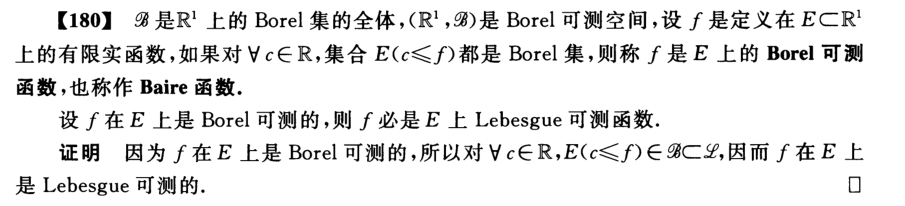
\includegraphics[width=\textwidth]{积分理论-2025040600.png}
% \caption{}
\label{}
\end{figure}
\end{definition}
\begin{exercise}[Baire 函数很接近有限的 Lebesgue 可测函数]
设 $f$ 是 $E\in \mathcal{R}$ 上有限的 Lebesgue 可测函数,则一定存在全直线 $\mathbb{R}^{1}$ 上的 Borel 可测函数 $h$ 使得
\[
m(E(f\neq h))=0
\]
\end{exercise}
\begin{proof}
\begin{figure}[H]
\centering
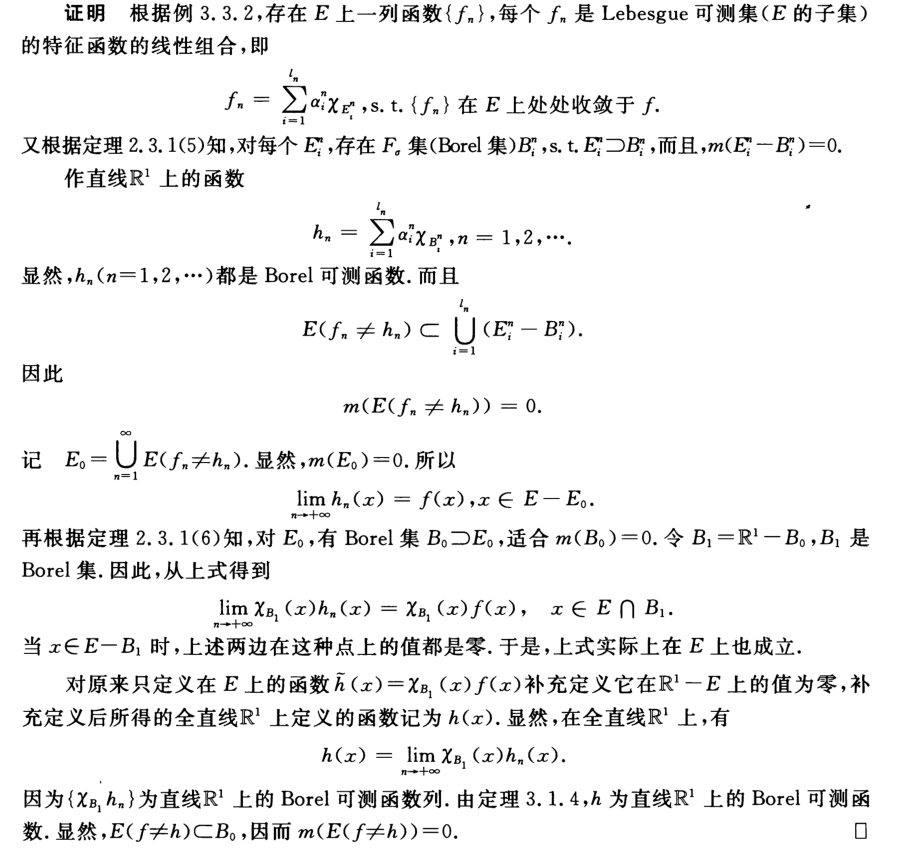
\includegraphics[width=\textwidth]{1-积分理论-2025040600.png}
% \caption{}
\label{}
\end{figure}
\end{proof}

\section{积分理论}

\begin{theorem}[Levi 定理]
设 $(X,\mathcal{R},\mu)$ 为测度空间,$\{ f_k \}$ 为 $E\in \mathcal{R}$ 上的非负广义可测递增函数列,且 $\lim_{ k \to \infty }f_k (x)=f (x),\forall x\in E$. 则
\[
\lim_{ k \to \infty } \int_{E}^{} f_k \, \mathrm{d}\mu=\int_{E}^{} f \, \mathrm{d}\mu=\int_{E}^{} \lim_{ k \to \infty } f_k \, \mathrm{d}\mu  
\]
\end{theorem}
\begin{exercise}
$f$ 为 Lebesgue 可测集 $E\subset \mathbb{R}^{n}$ 上的几乎处处大于零的 Lebesgue 可测函数,且满足
\[
\int_{E}^{} f \, \mathrm{d}m =0
\]
证明:$m(E)=0$.
\end{exercise}
\begin{proof}
考虑反证,我们知道
\[
E=E(f\leq 0)\bigcup\left( \bigcup_{k=1}^{\infty} E\left( f\geq \frac{1}{k} \right) \right)
\]
由题意 $m(E(f\leq0))=0$,若 $m(E)>0$ 则存在 $k_0$ 使得 $m\left( E\left( f\geq\frac{1}{k_0} \right) \right)>0$,那么
\[
0=\int_{E}^{} f \, \mathrm{d}m\geq \int_{E\left( f\geq \frac{1}{k_0}  \right)}^{} f  \, \mathrm{d}m\geq \frac{1}{k_0}m\left( E\left( f\geq \frac{1}{k_0}  \right) \right)>0
\]
矛盾!

\end{proof}

\begin{exercise}
设 $f$ 为 $E\subset \mathbb{R}^{n}$ 上非负 Lebesgue 可积函数
\[
E_k\coloneqq \{ x\in E :f(x)\geq k\}\qquad k=1,2,\dots
\]
证明:$\sum_{k=1}^{\infty}m(E_k)<+\infty$.
\end{exercise}
\begin{proof}
记 $F_k=\{ x\in E:k\leq f(x)<k+1 \},k=0,1,\dots$, 则 $E=\bigsqcup_{k=0}^{\infty}F_k$,于是
\[
\begin{aligned}
+oo & \overset{ f\in L^{1} }{ > } \int_{E}^{} f \, \mathrm{d}m =\sum_{k=0}^{\infty} \int_{F_k}^{} f \, \mathrm{d}m\geq \sum_{k=0}^{\infty} k\cdot m(F_k) \\
 & =[m(F_1)+m(F_2)+m(F_3)+\dots]+[m(F_2)+m(F_3)+\dots]+\dots \\
 & =\sum_{k=1}^{\infty} m(E_k)
\end{aligned}
\]
\end{proof}

\begin{exercise}
设 $f$ 为 $E \subset \mathbb{R}^n$ 上的 Lebesgue 可测函数,$m(E)<+\infty$ .证明:
$f^2$ 为 $E$ 上的 Lebesgue 可积函数 $\Leftrightarrow \sum_{k=1}^{\infty} k \cdot m(\{x \in E| | f(x) \mid>k\})<+\infty$ .如果 $m(E)=+\infty$ ,举例说明充分性不成立.
\end{exercise}
\begin{proof}

令 $E_k=\{x \in E| | f(x) \mid>k\}$ ,则
\[
\begin{aligned}
& k^2\left[m\left(E_k\right)-m\left(E_{k+1}\right)\right] \leqslant \int_{E_k-E_{k+1}} f^2 \mathrm{~d} m \leqslant(k+1)^2\left[m\left(E_k\right)-m\left(E_{k+1}\right)\right], \\
& \sum_{k=0}^{\infty} k^2\left[m\left(E_k\right)-m\left(E_{k+1}\right)\right] \leqslant \int_E f^2 \mathrm{~d} m \leqslant \sum_{k=0}^{\infty}(k+1)^2\left[m\left(E_k\right)-m\left(E_{k+1}\right)\right], \\
& \sum_{k=1}^{\infty} k m\left(E_k\right) \leqslant \sum_{k=0}^{\infty}(2 k+1) m\left(E_{k+1}\right) \leqslant \int_E f^2 \mathrm{~d} m \leqslant \sum_{k=0}^{\infty}(2 k+1) m\left(E_k\right) \\
& \leqslant 3 \sum_{k=1}^{\infty} k m\left(E_k\right)+m\left(E_0\right) \leqslant 3 \sum_{k=1}^{\infty} k m\left(E_k\right)+m(E) .
\end{aligned}
\]
由此推得
$f^2$ 在 $E$ 上 Lebesgue 可积 $\Leftrightarrow \sum_{k=1}^{\infty} k m\left(E_k\right)=\sum_{k=1}^{\infty} k \cdot m(\{x \in E| | f(x) \mid>k\})<+\infty$ .

举出反例:$f (x)=1,\forall x\in E=\mathbb{R}^{n}$. 于是 $\sum km(E_k)=0$ 但是 $f\not\in L^2(E)$.
\end{proof}

\begin{exercise}
设
\[
\int_{0}^{2\pi} \lvert f(x) \rvert \cdot \ln(1+\lvert f(x) \rvert ) \, \mathrm{d}x <+\infty
\]
证明:$f\in L([0,2\pi])$.
\end{exercise}
\begin{proof}
设 $E_1=\{ x\in[0,2\pi]:\lvert f(x) \rvert<e-1 \},E_2=\{ x\in[0,2\pi]:\lvert f(x) \rvert\geq e-1 \}$. 则当 $x\in E_2$ 时,
\[
\ln(1+\lvert f(x) \rvert )\geq \ln(1+e-1)=1
\]
于是
\[
\begin{aligned}
\int_{0}^{2\pi} \lvert f(x) \rvert  \, \mathrm{d}x  & \leq \int_{E_1}^{ } \lvert f(x) \rvert  \, \mathrm{d}x +\int_{E_2}^{} \lvert f(x) \rvert  \, \mathrm{d}x  \\
 & \leq (e-1)m(E_1)+\int_{E_2}^{ } \lvert f(x) \rvert \cdot \ln(1+\lvert f(x) \rvert ) \, \mathrm{d}x  \\
 & \leq (e-1)m(E_1)+\int_{0}^{2\pi} \lvert f(x) \rvert \cdot \ln(1+\lvert f(x) \rvert ) \, \mathrm{d}x <+\infty
\end{aligned}
\]
于是 $f\in L([0,2\pi])$.

\end{proof}

\section{勒贝格微分定理,勒贝格点}

\begin{theorem}[勒贝格微分定理]
设 $f \in L_{\mathrm{loc}}^{1}\left(\mathbb{R}^{d}\right)$, 则对于几乎处处的 $x \in \mathbb{R}^{d}$, 我们有
\[
\lim _{r \rightarrow 0} \frac{1}{m(B(x, r))} \int_{B(x, r)} f(y) d y=f(x) .
\]
\end{theorem}
\begin{definition}[Lebesgue 点]
设 $f \in L_{loc}^1\left(\mathbb{R}^n\right)$. 对 $\mathbb{R}^n$ 中的 $x$, 如果
\[
\lim _{r \rightarrow 0} \frac{1}{|B(x, r)|} \int_{B(x, r)}|f(y)-f(x)| d y=0,
\]那么称 $x$ 为 $f$ 的 \textbf{Lebesgue 点}.
\end{definition}
若 $f\in L^{1}_{\text{loc}}(E)$ ,那么 $E$ 几乎处处为 $f$ 的 Lebesgue 点.
